\textbf{11.2}
\begin{itemize}
\item[(a)]
  Use the method of lines and an ODE solver of your choice to solve the heat equation
  \begin{displaymath}
    u_t = u_{xx}, \quad 0\le x \le 1, \quad t\ge 0,
  \end{displaymath}
  with initial condition
  \begin{displaymath}
    u(0, x) = \sin(\pi x), \quad 0\le x \le 1,
  \end{displaymath}
  and Dirichlet boundary conditions
  \begin{displaymath}
    u(t, 0) = 0, \quad u(t, 1) = 0, \quad t\ge 0.
  \end{displaymath}
  Integrate from $t=0$ to $t=0.1$.
  Plot the computed solution,
  preferably as a three-dimensional surface over the $(t, x)$ plane.
  If you do not have three-dimensional plotting capability,
  plot the solution as a function of $x$ for a few values of $t$,
  including the initial and final times.
  Determine the maximum error in the computed solution by
  comparing with the exact solution
  \begin{displaymath}
    u(t, x) = \exp(-\pi^2t)\sin(\pi x).
  \end{displaymath}
  Experiment with various spatial mesh sizes $\Delta x$,
  and try to characterize the error as a function of $\Delta x$.
  On a log-log scale,
  plot the maximum error as a function of $\Delta x$.

\item[(b)]
  Repeat part (a),
  but this time with initial condition
  \begin{displaymath}
    u(0, x) = \cos(\pi x), \quad 0\le x \le 1,
  \end{displaymath}
  and Neumann boundary conditions
  \begin{displaymath}
    u_x(t, 0) = 0, \quad u_x(t, 1) = 0, \quad t\ge 0,
  \end{displaymath}
  and compare with the exact solution.
\end{itemize}
\begin{itemize}
\begin{multicols}{2}
  \setlength{\columnseprule}{0.2pt}
  \item[(a)]
    Discretize the spatial domain
    \begin{displaymath}
      x_i = i\Delta x, \quad i=0, 1, \ldots, m+1,
    \end{displaymath}
    where the spatial mesh size $\Delta x=\frac{1}{m+1}$.
  Discretizing the heat equation with respect to spatial variables only,
  we obtain
  \begin{displaymath}
    \frac{\dif u_i(t)}{\dif t} = \frac{u_{i-1}(t)-2u_i(t)+u_{i+1}(t)}{(\Delta x)^2},
    \quad i=1, \ldots, m,
  \end{displaymath}
  and
  \begin{displaymath}
    u_i(0) = \sin(\pi i\Delta x), \quad i=1, \ldots, m,
  \end{displaymath}
  the Dirichlet boundary conditions are discretized into
  \begin{displaymath}
    u_0(t) = 0, \quad u_{m+1}(t) = 0, \quad t\ge 0.
  \end{displaymath}
  The code is shown as follows.

  \verb|func_mol.m|
  \lstinputlisting[firstnumber=1]{matlab/func_mol.m}

  \verb|mol.m|
  \lstinputlisting[firstnumber=1]{matlab/mol.m}
\end{multicols}

\begin{figure}[H]
  \centering
  \subfigure[$m = 10$]{
    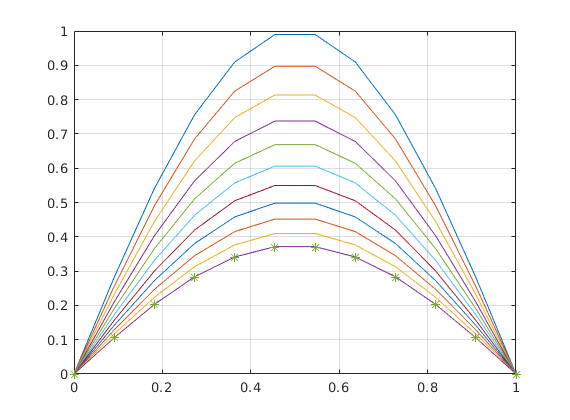
\includegraphics[width=0.305\linewidth]{png/m10}
  }
  \hfill
  \subfigure[$m = 20$]{
    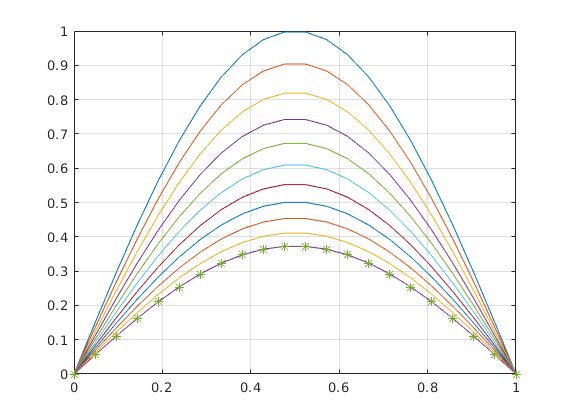
\includegraphics[width=0.305\linewidth]{png/m20}
  }
  \hfill
  \subfigure[$m = 40$]{
    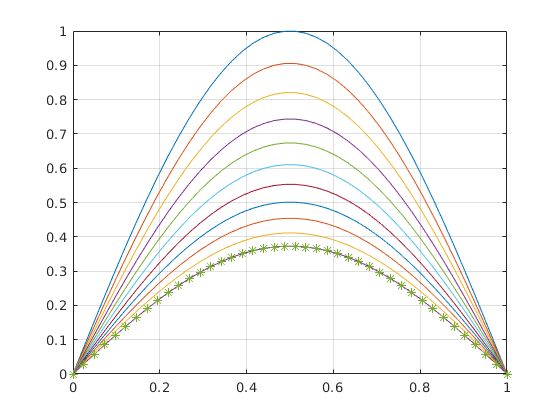
\includegraphics[width=0.305\linewidth]{png/m40}
  }
  \hfill
  \subfigure[$m = 80$]{
    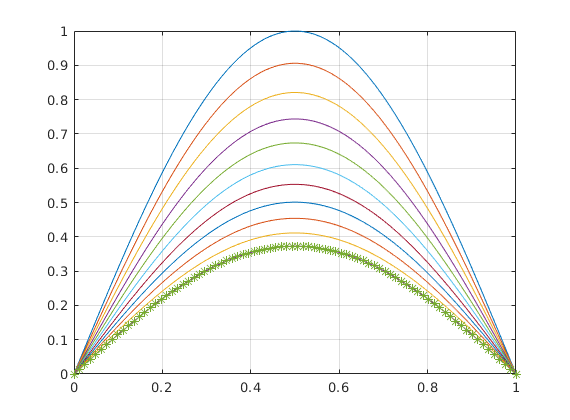
\includegraphics[width=0.305\linewidth]{png/m80}
  }
  \hfill
  \subfigure[$m = 160$]{
    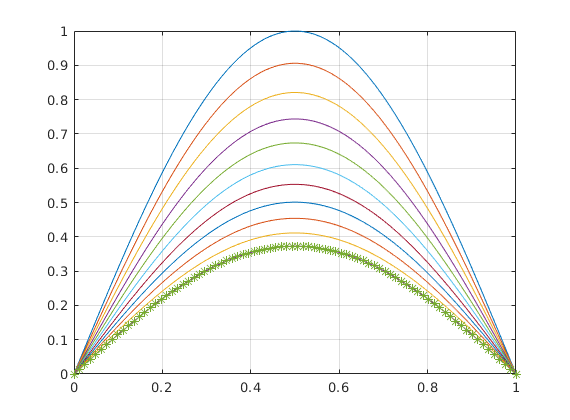
\includegraphics[width=0.305\linewidth]{png/m160}
  }
  \hfill
  \subfigure[$m = 320$]{
    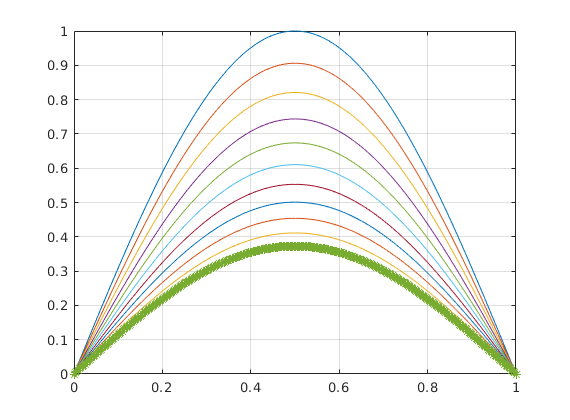
\includegraphics[width=0.305\linewidth]{png/m320}
  }
\end{figure}
  To characterize the error as a function of $\Delta x$,
  we modify the ODE solver used in \verb|mol.m| as follows.
\begin{verbatim}
options = odeset('RelTol',1e-9,'AbsTol',1e-12);
[t,u] = ode23s('func_mol',[t0, tfinal],y0,options);
\end{verbatim}

  On a log-log scale,
  the maximum error as a function of $\Delta x$ is as illustrated by the following figure.
  \begin{figure}[H]
    \centering
    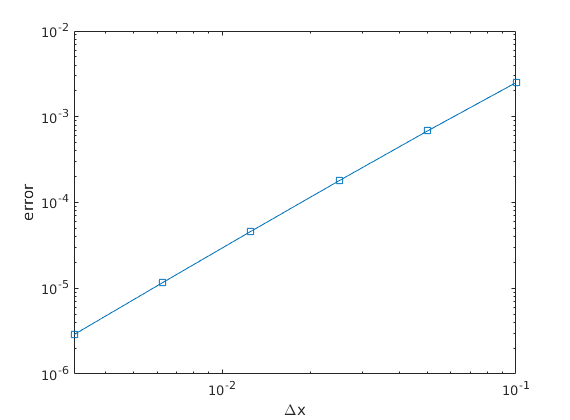
\includegraphics[scale=0.55]{png/err.png}
  \end{figure}

\item[(b)]
  \begin{multicols}{2}
    \setlength{\columnseprule}{0.2pt}
  In this case,
  the discretization of the heat equation is
  \begin{align*}
    \frac{\dif u_0(t)}{\dif t} &= \frac{-2u_0(t)+2u_1(t)}{(\Delta x)^2}, \\
    \frac{\dif u_i(t)}{\dif t} &= \frac{u_{i-1}(t)-2u_i(t)+u_{i+1}(t)}{(\Delta x)^2}, i = 1,\ldots, m, \\
    \frac{\dif u_{m+1}(t)}{\dif t} &= \frac{2u_m(t)-2u_{m+1}(t)}{(\Delta x)^2},
  \end{align*}
  with initial condition
  \begin{displaymath}
    u_i(0) = \cos(\pi i\Delta x), \quad i=1, \ldots, m.
  \end{displaymath}
  The code is shown as follows.

    \verb|func_mol2.m|
  \lstinputlisting[firstnumber=1]{matlab/func_mol2.m}

  \verb|mol2.m|
  \lstinputlisting[firstnumber=1]{matlab/mol2.m}
\end{multicols}

\begin{figure}[H]
  \centering
  \subfigure[$m = 10$]{
    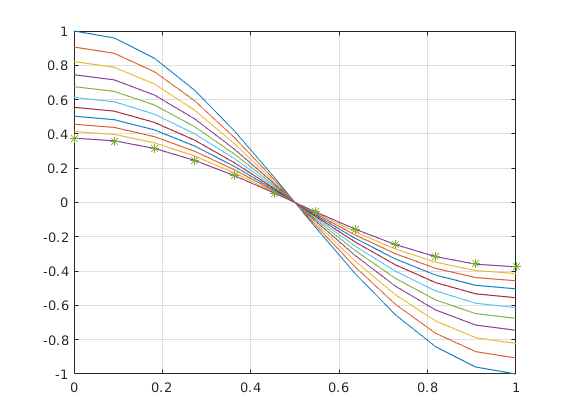
\includegraphics[width=0.305\linewidth]{png/2m10}
  }
  \hfill
  \subfigure[$m = 20$]{
    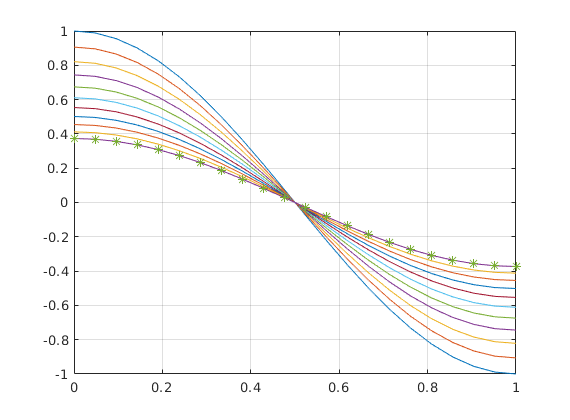
\includegraphics[width=0.305\linewidth]{png/2m20}
  }
  \hfill
  \subfigure[$m = 40$]{
    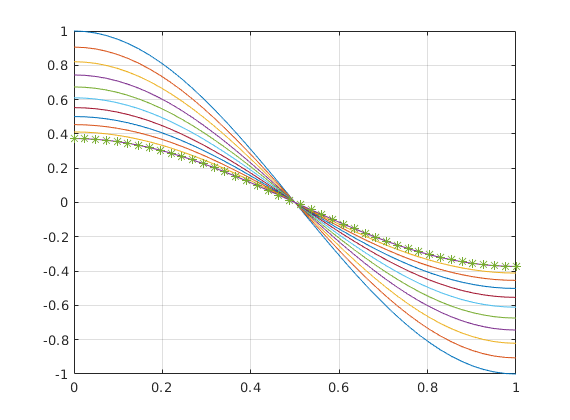
\includegraphics[width=0.305\linewidth]{png/2m40}
  }
  \hfill
  \subfigure[$m = 80$]{
    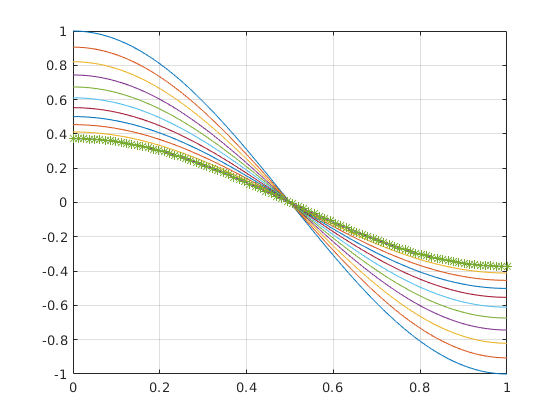
\includegraphics[width=0.305\linewidth]{png/2m80}
  }
  \hfill
  \subfigure[$m = 160$]{
    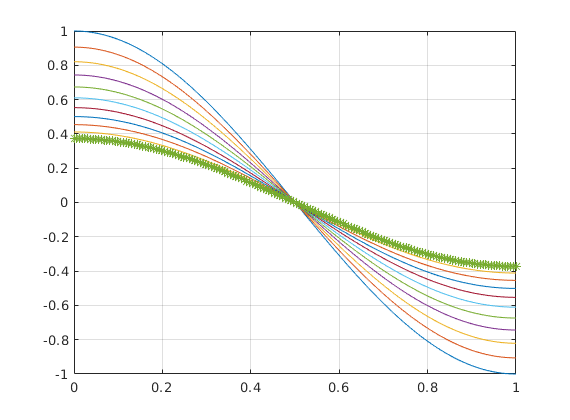
\includegraphics[width=0.305\linewidth]{png/2m160}
  }
  \hfill
  \subfigure[$m = 320$]{
    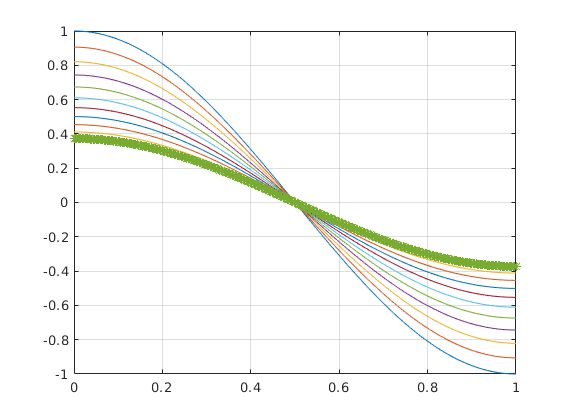
\includegraphics[width=0.305\linewidth]{png/2m320}
  }
\end{figure}
  To characterize the error as a function of $\Delta x$,
  we modify the ODE solver used in \verb|mol2.m| as follows.
\begin{verbatim}
options = odeset('RelTol',1e-9,'AbsTol',1e-12);
[t,u] = ode23s('func_mol',[t0, tfinal],y0,options);
\end{verbatim}

  On a log-log scale,
  the maximum error as a function of $\Delta x$ is as illustrated by the following figure.
  \begin{figure}[H]
    \centering
    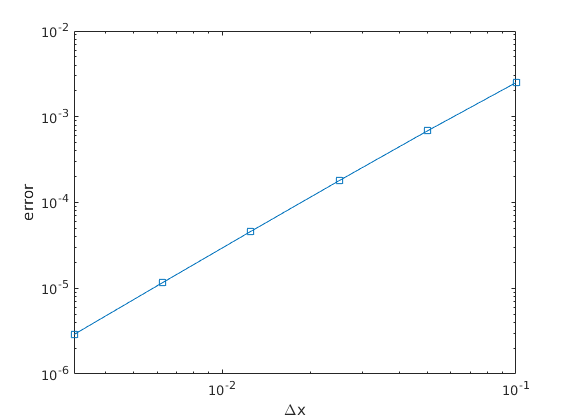
\includegraphics[scale=0.55]{png/herr2.png}
  \end{figure}
\end{itemize}
%%% Local Variables:
%%% mode: latex
%%% TeX-master: "../ComputerAssignment"
%%% End:
